\chapter{Methods}
\graphicspath{{chapters/methods/}}

\section{Dense Linear Algebra}
\subsection{Dense Linear Algebra Applications}
\subsection{Block-Based LU factorization}

\begin{algorithm}[h]
	\DontPrintSemicolon
	%\SetAlgoVlined
	\caption{LU Factorization\label{alg:lufact}}
	\For{k \KwFrom 0 \KwTo p-2}{
		(1) $\displaystyle Inv^{(k)} = [A_{k,k}^{(k)}]^{-1}$ \;
		\For{i \KwFrom k+1 \KwTo p-1}{
			(2) $\displaystyle A_{i,k}^{(k+1)} = A_{i,k}^{(k)} \cdot Inv^{(k)}$ \;
			\For{j \KwFrom k+1 \KwTo p-1}{
				(3) $A_{i,j}^{(k+1)} = A_{i,j}^{(k)} - A_{i,k}^{(k+1)} \cdot A_{k,j}^{(k)}$ \;
			}
		}
	}
\end{algorithm}


\subsection{Block-Based Gaussian Elimination to Solve Linear Systems}

\begin{algorithm}[h]
	\DontPrintSemicolon
	\caption{Block-Based Gaussian elimination and back substitution \label{alg:bg_el}}
	%\scriptsize
	\For{k \KwFrom 0 \KwTo p-2}{
		(1) $\displaystyle Inv^{(k)} = [A_{k,k}^{(k)}]^{-1}$ \;
		(2) $b_k^{(k+1)} = Inv^{(k)} \cdot b_k^{(k)}$ \;
		\For{j \KwFrom k+1 \KwTo p-1}{
			(3) $\displaystyle A_{k,j}^{(k+1)} = Inv^{(k)} \cdot A_{k,j}^{(k)} $ \;
		}
		\For{i \KwFrom k+1 \KwTo p-1}{
			(4) $b_i^{(k+1)} = b_i^{(k)} - A_{i,k}^{(k)} \cdot b_k^{(k+1)}$ \;
			\For{j \KwFrom k+1 \KwTo p-1}{
				(5) $A_{i,j}^{(k+1)} = A_{i,j}^{(k)} - A_{i,k}^{(k)} \cdot A_{k,j}^{(k+1)}$ \;
			}
		}
	}

	(6) $b_{p-1}^{(p)} = Inv^{(p-1)} \cdot b_{p-1}^{(p-1)}$ \;

	\For{k \KwFrom 1 \KwTo p-1 }{
		\For{i \KwFrom 0 \KwTo p-k-1 }{
			(7) $b_i^{(k+i+1)} = b_i^{(k+i)} - A_{i,p-k}^{(i+1)} \cdot b_{p-k}^{(p)}$ \;
		}
	}
\end{algorithm}

\subsection{Block-Based Gauss-Jordan Elimination to Solve Linear Systems}

\begin{algorithm}[h]
	\DontPrintSemicolon
	\caption{Block-Based Gauss-Jordan elimination to solve a linear system \label{alg:bgj} }
	\For{k \KwFrom 0 \KwTo p-1}{
		(1) $\displaystyle Inv^{(k)} = [A_{k,k}^{(k)}]^{-1}$ \;
		(2) $b_k^{(k+1)} = Inv^{(k)} \cdot b_k^{(k)}$ \;
		\For{j \KwFrom k+1 \KwTo p-1}{
			(3) $\displaystyle A_{k,j}^{(k+1)} = Inv^{(k)} \cdot A_{k,j}^{(k)} $ \;
			\For{i \KwFrom 0 \KwTo p-1}{
				\If{k $\neq$ i}{
					(4) $A_{i,j}^{(k+1)} = A_{i,j}^{(k)} - A_{i,k}^{(k)} \cdot A_{k,j}^{(k+1)}$ \;
				}
			}
		}
		\For{i \KwFrom 0 \KwTo p-1}{
			\If{k $\neq$ i}{
				(5) $b_i^{(k+1)} = b_i^{(k+1)} - A_{i,k}^{(k)} \cdot b_k^{(k+1)}$ \;
			}
		}
	}
\end{algorithm}

\subsection{Block-Based LU factorization to Solve Linear Systems}


\begin{algorithm}[h]
	\DontPrintSemicolon
	%\SetAlgoVlined
	\caption{Solution of a linear system with a block-based LU factorization\label{alg:lufact_sls}}
	\For{i \KwFrom 0 \KwTo p-2}{
		\For{j \KwFrom i+1 \KwTo p}{
			(5) $b_j^{(i+1)} = b_j^{(i)} - A_{j,i}^{(i+1)} \cdot b_i^{(p)}$ \;
		}
	}
	\;
	\For{k \KwFrom p-1 \KwTo 0 \KwStep -1}{
		(6) solve $b_{k}^{(p)} = A_{k,k}^{(k)} \cdot b_k^{(p-1)}$ \;
		\For{i \KwFrom 1 \KwTo k-1}{
			(7) $b_i^{(p-k+i)} = b_i^{(p-k+i-1)} - A_{i,k}^{(i)} \cdot b_k^{(p)}$ \;
		}
	}
\end{algorithm}


ccl : physical simulation can produce sparse matrices to save space and computations \dots
\section{Sparse Linear Algebra}

\subsection{Sparse Matrix Applications}
\subsection{Sparse Matrix Storage and Sparse Matrix-Vector Multiplication}

\subsubsection{Dense}
\subsubsection{Coordinates - COO}
\subsubsection{Compressed Sparse Row - CSR}
\subsubsection{Diagonal - DIA}
\subsubsection{Ellpack-Itpack - ELL}
\subsubsection{Sparse General Pattern - SGP}
\subsubsection{Hybrid - HYB}
\subsection{Sparse Matrix-Vector Parallelization}
\subsection{Sparse Matrix-Vector Optimizations}
\subsection{Sparse $A(Ax + x) + x$}
\subsection{Test Matrices}


\section{Kirchhoff seismic pre-stack depth migration}

This section will present the Kirchhoff migration and continue the previous work made in \cite{rapport_Total_Petiton}.
This report explain the migration and gives hint to implement new algorithms for the migration.
This work take advantage from the discussions with Henri Calandra.
This section will detail the steps for the Kirchhoff migration.

\subsection{Overview}
The seismic migration is a technique used to visualize the underground.
Data are acquired at the surface during an acquisition campaign.
Data are processed to geometrically re-locate seismic events either in space or in time.
They are re-located to the location the event occurred in the subsurface rather than the location where it was recorded at the surface.
Migration moves dipping reflectors to their true subsurface positions and collapses diffractions, resulting in a migrated image that typically has an increased spatial resolution and resolves areas of complex geology much better than non-migrated images.
A form of migration is one of the standard data processing techniques for reflection-based geophysical methods (seismic reflection and ground-penetrating radar).

The Kirchhoff migration \cite{PingY1995} \cite{PTSCS2009} is a depth migration.
It is applied to seismic data in depth (regular Cartesian) coordinates, which must be calculated from seismic data in time coordinates.
This method does therefore require a velocity model, making it resource-intensive because building a seismic velocity model is a long and iterative process (Figure \ref{fig:kirchhoff-process}).
The significant advantage to this migration method is that it can be successfully used in areas with lateral velocity variations, which tend to be the areas that are most interesting to petroleum geologists.

\begin{figure}[H]
	\centering
	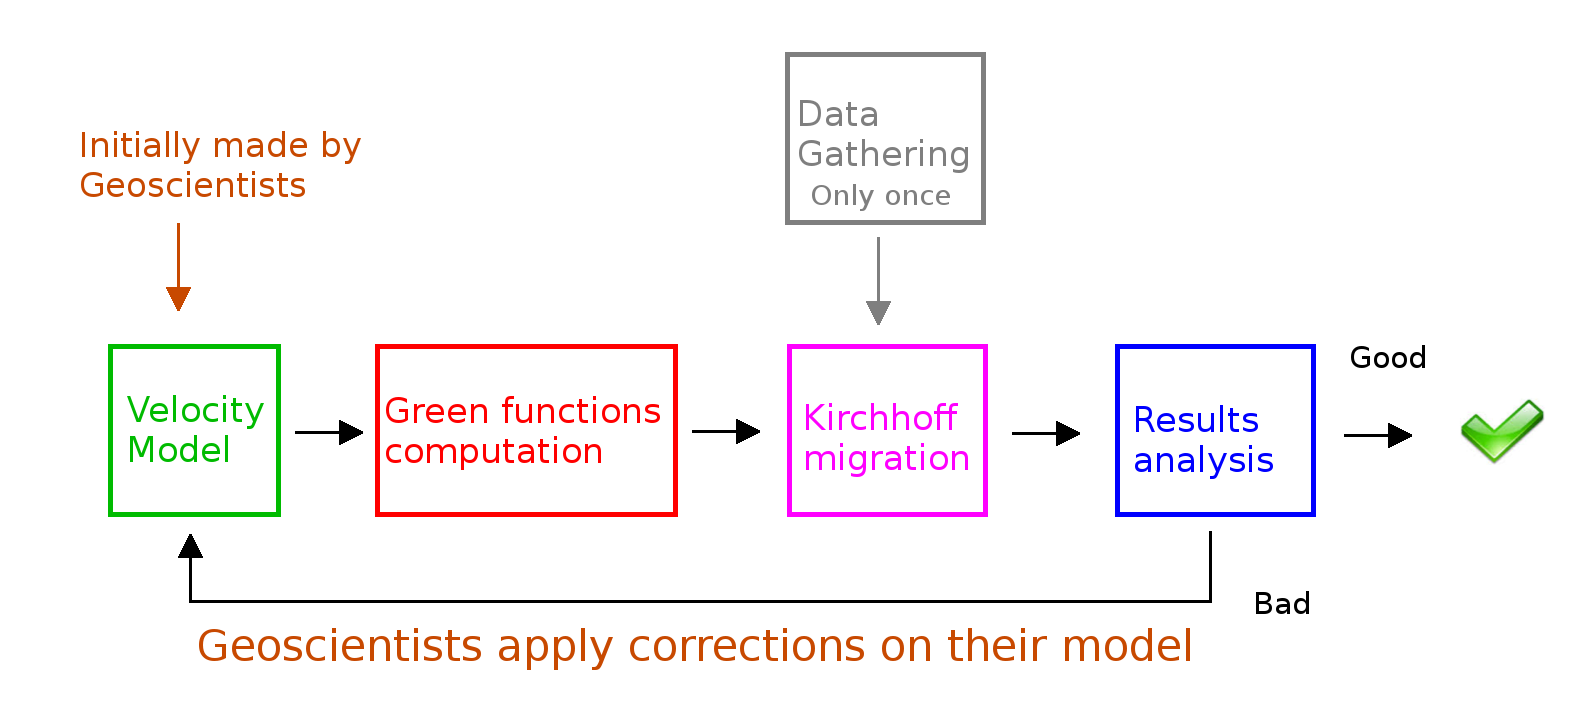
\includegraphics[scale=0.25]{kirchhoff-process}
	\caption{Building process of a seismic velocity model \label{fig:kirchhoff-process}}
\end{figure}

\subsection{Velocity model}
The velocity model describe the propagation speed of the waves into the different layer of the underground.
Geophysicists create a model and want to verify its correctness.
Their goal is to find the best model that explain the data.
They use the Kirchhoff migration that determine where are the limits between layers.
This method processes data called traces.
They are the output from a seismogram (receiver) at the surface after the emission (source) of a wave into the ground.
If the model is coherent with the image generated by the migration, the model is correct.
Otherwise, the model is adjusted by geophysicists and the migration is re-used to obtain a new image.
This process is repeated until the image and the model are coherent.

\subsection{Data gathering}
Data are produced during an acquisition campaign.
A campaign contains several shots.
A shot is a seismic impulsion launched through the ground.
It is the source (see Figure \ref{fig:shot}).
There is several receiver.
They are seismograms placed on a 2D grid on the ground (see Figure \ref{fig:source-receiver}).
The source is moved on the 2D grid and produces shots.
So a trace is the result for a given shot (source) and a given seismogram (receiver).

\begin{figure}[H]
	\centering
	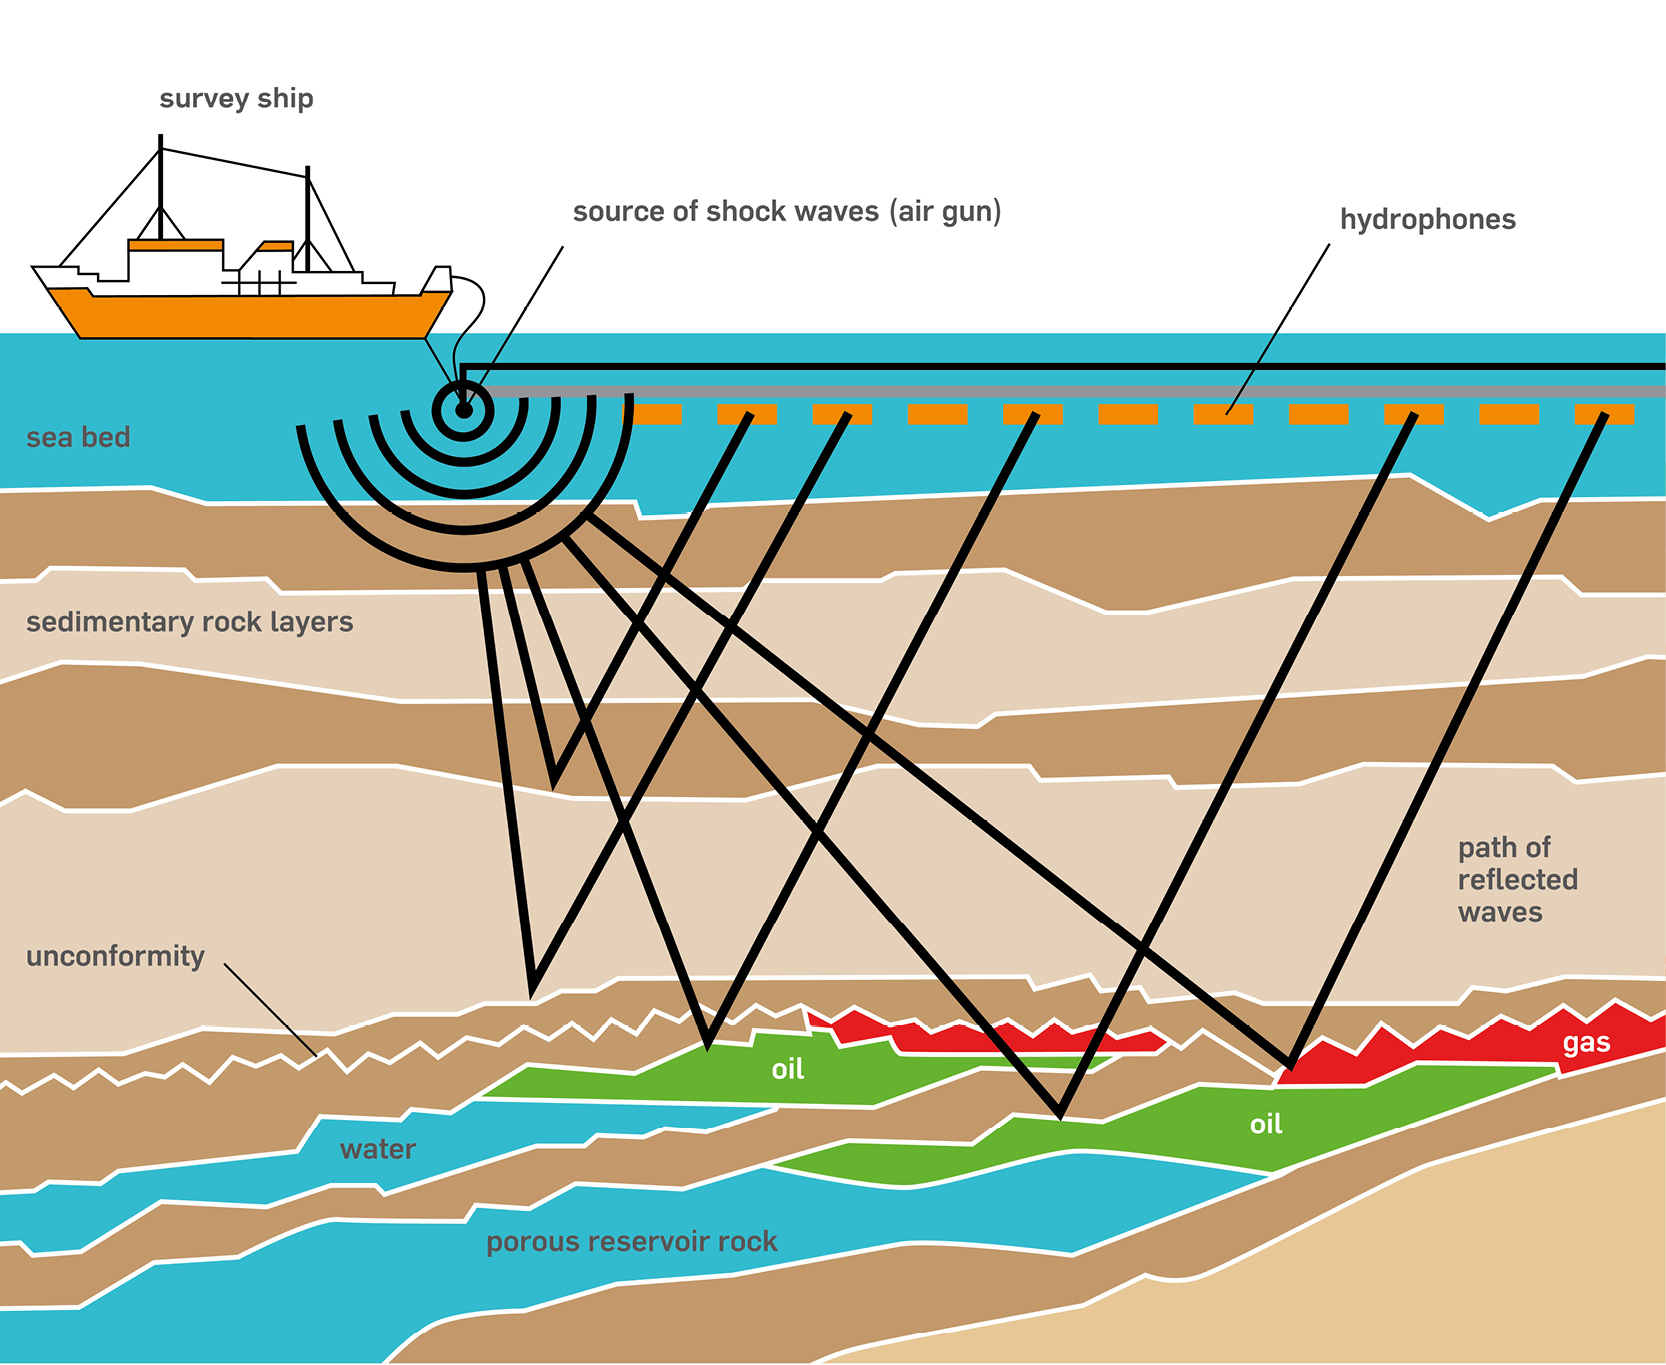
\includegraphics[scale=0.75]{oss}
	\caption{Shot during Data acquisition \label{fig:shot}}
\end{figure}
\begin{figure}[H]
	\centering
	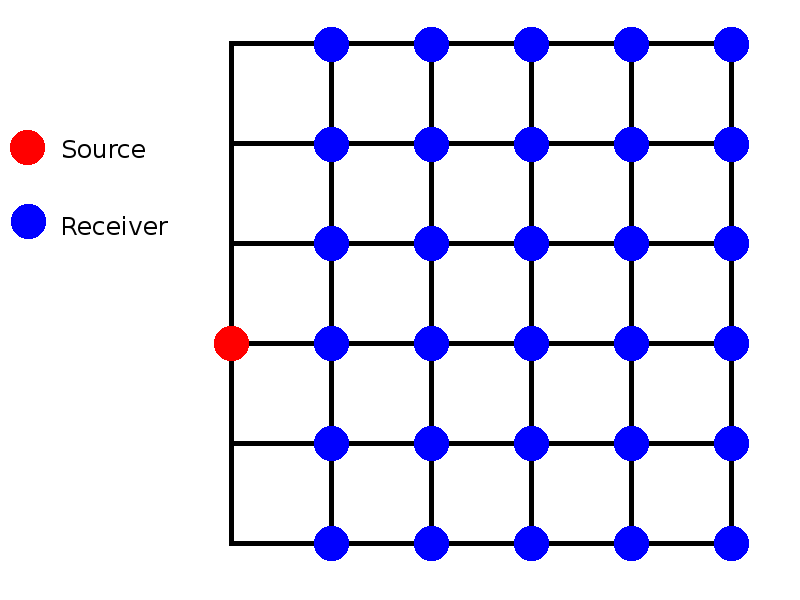
\includegraphics[scale=0.37]{gridSR}
	\caption{Shot and seismograms \label{fig:source-receiver}}
\end{figure}

The acquisition campaign gives a huge amount of traces since there is a lot of receiver and several shots.
A trace contains the coordinates of the source and the receiver and the data from the seismogram.

\subsection{Green functions}
The Green functions represent the response and the behaviour of the wave when the source is a Dirac impulse.
They allow to solve the wave equation using an integral formula in function of the source of the wave.
The behaviour of the wave in the ground depends on the velocity model.
Usually, Green functions are pre-calculated and stored on disk for a 2D grid on surface and a 3D grid underground.
During the building of the model and the migration, Green functions are retrieved from disk.

In the Kirchhoff migration, the Green functions are used to estimate the travel time between 2 points depending on the velocity model.
We estimate the travel time between a source S and a point P of the image ($T_{SP}$) then between P and a receiver R ($T_{PR}$).
So we can deduce $T_{SPR} = T_{SP} + T_{PR}$ (see Figure \ref{fig:Green_functions1}).

\begin{figure}[H]
	\centering
	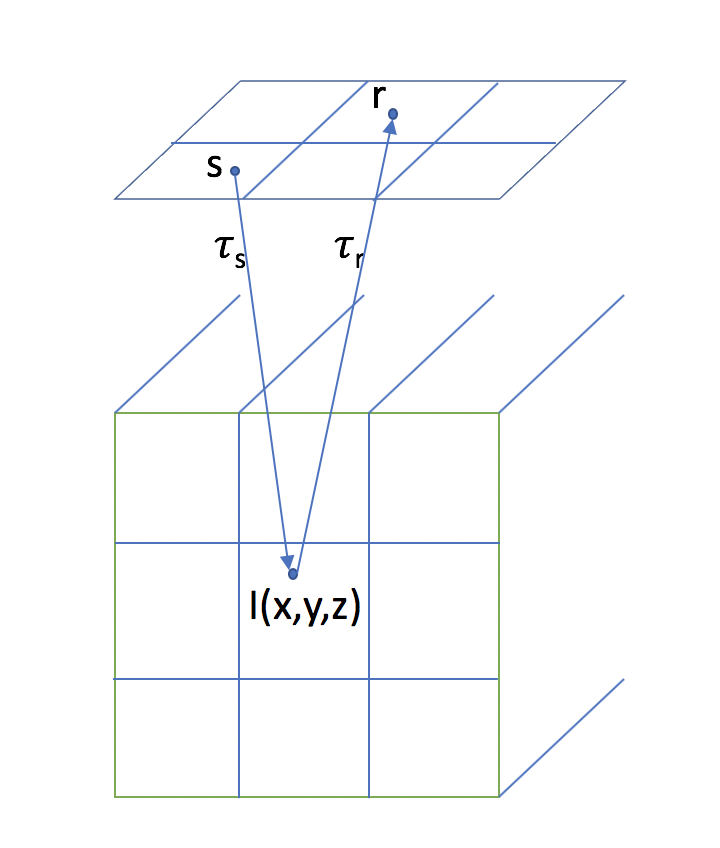
\includegraphics[scale=0.6]{img1}
	\caption{Wave travel between S and R through P\label{fig:Green_functions1} from \cite{rapport_Total_Petiton}}
\end{figure}

Green functions are pre-calculated for a 2D grid at the surface and for à 3D grid underground (see Figure \ref{fig:grids}).
Moreover, a block of the 3D grid contains an image at a finer grain.
Therefore, it is necessary to interpolate or extrapolate the Green functions for the points into the finer grid (see Figure \ref{fig:fine_coarse_grid}).

\begin{figure}[H]
	\centering
	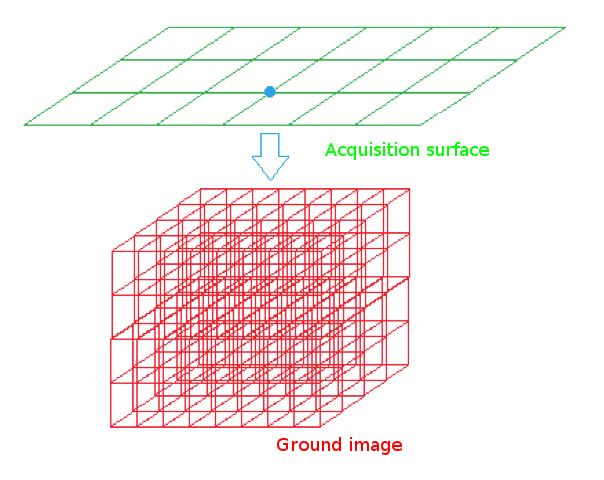
\includegraphics[width=.55\textwidth]{figure8rapportP2}
	\caption{2D and 3D grids \label{fig:grids} from \cite{rapport_Total_Petiton}}
\end{figure}

\begin{figure}[H]
	\centering
	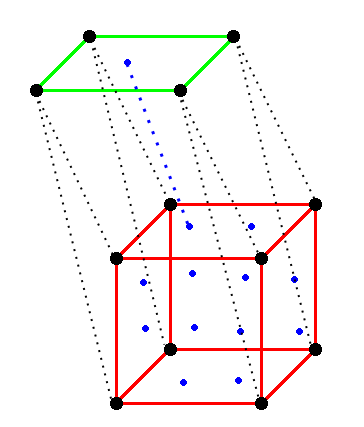
\includegraphics[width=.55\textwidth]{fctGreenInterpolation}
	\caption{Coarse grid and points from the finer grid \label{fig:fine_coarse_grid}}
\end{figure}

\subsection{Kirchhoff migration \label{sec:kirchhoff}}
The Kirchhoff migration produces a 3D image of the subsurface by retrieving the position of the reflection points in order to show the different layers of the ground.
To do so, find the time a wave need to travel from a source to a point $(x,y,z)$ in the image and travel back from this point to the receiver is necessary.
The Green functions in the fine grid give this time.
Then, the trace\footnote{http://www.iris.washington.edu/ds/nodes/dmc/manuals/irisfetchm/} (Figure \ref{fig:kir_trace}) has a peak when the wave arrives to the receiver.
This corresponds to the time it needs for the trace to travel from the source to the receiver into the ground.
For a given source and receiver, if the time a wave need to travel trough the point $(x,y,z)$ and the time to the peak of the trace match then $(x,y,z)$ can be a candidate to a reflection point.

\begin{figure}[H]
	\centering
	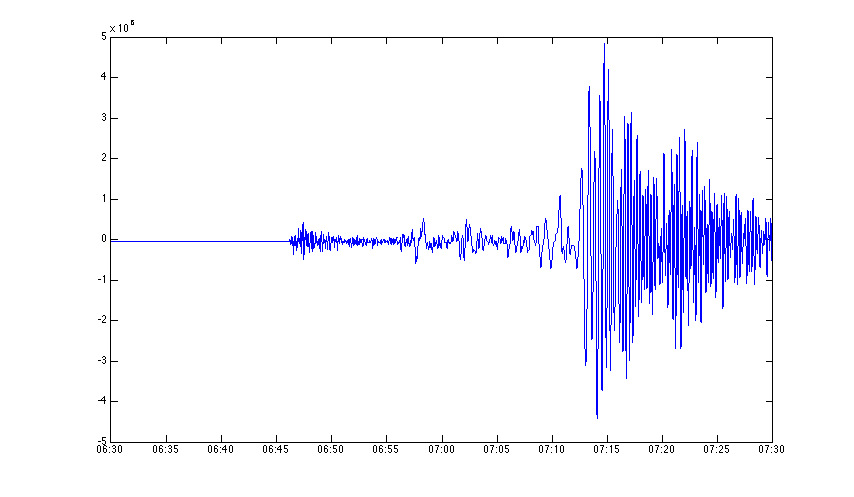
\includegraphics[width=.75\textwidth]{trace}
	%http://www.iris.washington.edu/ds/newsletter/vol14/no1/7/direct-data-access-from-within-matlab/
	\caption{A trace from the IRIS-DMC repository\label{fig:kir_trace}}
\end{figure}

Moreover, we know the Green functions for a coarse grain of the image, so it is possible to know if the points in the sub-domain of the coarse grid will match the time from the trace.
If the time matches, the points will be studied at a finer grain.
Otherwise, the points of the part of the coarse grid will not be candidates to a reflection point and those points will be ignored for the selected trace.

At the finer grain level, when the block of coarse grid matches with the time of the trace, the Green functions are interpolated or extrapolated for each point in the block.
This give the travel time $T(x,y,z)$ between the source and the receiver passing by the point $(x,y,z)$.
Then, only the points matching the time of the trace are kept.
Those points are likely true reflection points.
An arbitrary value (the aperture) $A_{s,r}(x,y,z)$  \cite{XHCCC2014} that favours points with less awkward reflection angles, and positions that are more likely to match the true reflection point, can be calculated.
This value depends on the coordinates of the receiver 'r', the coordinates of the source 's' and the point $(x,y,z)$.
The value $A_{s,r}(x,y,z) t_{s,r}(x,y,z)$ expresses the intensity of the contribution of the trace for the point $(x,y,z)$.

The image at a point is generated by summing the contribution of all the traces that can be a true reflection point :


\begin{equation}
	I(x,y,z)=\sum_{t_{s,r} \in T}A_{s,r}(x,y,z)t_{s,r}(\tau_s(x,y,z) + \tau_r(x,y,z))
\end{equation}

$I(x,y,z)$ is the point $(x,y,z)$ of the image.
$t_{s,r}$ is the trace which has $s$ as source and $r$ as receiver.
$T$ is the ensemble of traces.
$A_{s,r}$ is the amplitude associated to $s$ and $r$.
$\tau_j(x,y,z)$  is the time need for a wave to travel from $j$ (a source or a receiver) to $(x,y,z)$.


In the existing application, the Green functions (the time needed by the sound wave to go from the source or the receiver to the point inside the grid, the values of $\tau$) are pre-computed from the velocity model which is evaluated and imported from the file system when the application is using them.

Moreover, two granularities of grids are used.
The values of $A$ and $\tau$ are computed for the coarse grid and they are interpolated from the computed values for the fine grid.


\subsection{Analysis of the results}
The resulting image is analysed by geophysicists.
If they think that the velocity model is coherent with the image, the model can be exploited.
Otherwise, the velocity model is modified and the process of the Kirchhoff migration is reused until the geophysicists judge that the velocity model corresponds to the data.